% SBB-roter Abschlussbericht (article, pdfLaTeX)
\documentclass[12pt,oneside]{article}

% Sprache und Encodings
\usepackage[ngerman]{babel}
\usepackage[utf8]{inputenc}
\usepackage[T1]{fontenc}

% Schrift: serifenloser Hauptfont (Helvetica/TeX Gyre Heros Ersatz)
\renewcommand{\familydefault}{\sfdefault}
\usepackage{helvet} % setzt die serifenlose Schrift für pdfLaTeX

% Farben (angenommenes SBB-Rot)
\usepackage{xcolor}
\definecolor{sbbred}{HTML}{E2001A}
\definecolor{sbbgray}{HTML}{4D4D4D}

% Layout
\usepackage[a4paper, left=3cm, right=2.5cm, top=3cm, bottom=3cm]{geometry}
\usepackage{setspace}
\onehalfspacing

% Mikrotypografie (nur teilweise wirksam unter pdfLaTeX)
\usepackage{microtype} 

% Grafiken, Tabellen, etc.
\usepackage{graphicx}
\usepackage{caption}
\usepackage{subcaption}
\usepackage{booktabs}
\usepackage{longtable}
\usepackage{tabularx}
\usepackage{float}
\usepackage{pgfplots}
\pgfplotsset{compat=1.18}

% Kopf- und Fusszeilen
\usepackage{fancyhdr}
\pagestyle{fancy}
\fancyhf{}
\renewcommand{\headrulewidth}{0pt}
\fancyhead[L]{\color{sbbgray}\nouppercase{\leftmark}}
\fancyhead[R]{\color{sbbgray}\thepage}
\setlength{\headheight}{14pt}

% Hyperlinks
\usepackage{hyperref}
\hypersetup{
  colorlinks=true,
  linkcolor=sbbred,
  citecolor=sbbred,
  urlcolor=sbbred,
  pdftitle={Abschlussbericht},
  pdfauthor={Carina Santos}
}

% Code-Listings
\usepackage{listings}
\usepackage{courier}
\lstset{
  basicstyle=\ttfamily\small,
  keywordstyle=\color{sbbred}\bfseries,
  commentstyle=\color{sbbgray}\itshape,
  breaklines=true,
  numbers=left,
  numberstyle=\tiny
}

% Mathematik
\usepackage{amsmath,amssymb}

% Literatur: biblatex (backend=biber). Wenn du lieber BibTeX willst, siehe Hinweis unten.
\usepackage[backend=biber,style=authoryear,sorting=nyt]{biblatex}
\addbibresource{literatur.bib}

% Abkürzungsverzeichnis
\usepackage[printonlyused]{acronym}

% ----- Metadaten für Titelseite -----
\newcommand{\reporttitle}{Optimierte Schwellwertsetzung}
\newcommand{\reportauthor}{Dr. Carina Santos}
\newcommand{\reportdegree}{Praktikumsarbeit}
\newcommand{\reportdept}{SBB Energie}
\newcommand{\reportdate}{September 2026}
\newcommand{\reportsupervisor}{Betreuer: Dr. Andreas Fuchs}

% ----- Dokument -----
\begin{document}

% Titelseite (manuell gestaltet)
\begin{titlepage}
  \thispagestyle{empty}
  % oberer roter Balken mit Institutsname
  \vspace*{-1.5cm}
  \colorbox{sbbred}{%
    \parbox[b][3.0cm][c]{\dimexpr\textwidth+6cm\relax}{% verlängert bis zum Rand
      \hspace{1cm}\color{white}\Large\textbf{\reportdept}
    }%
  }

  \vspace{2.5cm}

  % Logo (falls vorhanden)
  \begin{center}
    \IfFileExists{images/sbb_logo.png}{%
      
\includegraphics[height=1.5cm]{images/sbb_logo.png}
    }{%
      \fbox{\parbox[c][6cm][c]{9cm}{\centering\color{sbbred}\textbf{SBB-Logo}}}
    }
  \end{center}

  \vspace{1.5cm}
  \begin{center}
    {\huge\bfseries \reporttitle \par}
    \vspace{1.2cm}
    {\Large \reportdegree \par}
    \vspace{2.5cm}
    {\Large \reportauthor \par}
    \vspace{0.6cm}
    {\large \reportsupervisor \par}
    \vspace{0.6cm}
    {\large \reportdate \par}
  \end{center}

  \vfill
  % Fuss-Balken
  \colorbox{sbbred}{%
    \parbox[b][0.8cm][c]{\dimexpr\textwidth+6cm\relax}{%
      \hspace{1cm}\color{white}\small SBB - Schweizerische Bundesbahnen
    }%
  }
\end{titlepage}

\clearpage
\pagenumbering{roman}

% Selbstständigkeitserklärung
\section*{Selbstständigkeitserklärung}
\addcontentsline{toc}{section}{Selbstständigkeitserklärung}
Hiermit versichere ich, dass ich die vorliegende Arbeit selbstständig und ohne unzulässige Hilfe Dritter angefertigt habe. Alle verwendeten Quellen und Hilfsmittel sind angegeben. Die Arbeit wurde bisher keiner anderen Prüfungsbehörde vorgelegt.

\vspace{2cm}
Ort, Datum:\\[1cm]
Unterschrift: \hrulefill

\clearpage

% Abstracts
\section*{Zusammenfassung}
\addcontentsline{toc}{section}{Zusammenfassung}
Kurzfassung auf Deutsch.

\section*{Abstract}
\addcontentsline{toc}{section}{Abstract}
Kurzfassung auf Englisch.

\clearpage
\tableofcontents
\listoffigures
\listoftables

\clearpage
\pagenumbering{arabic}
\setcounter{page}{1}

% Abkürzungen
\section*{Abkürzungsverzeichnis}
\addcontentsline{toc}{section}{Abkürzungsverzeichnis}
\begin{acronym}[SBB]
  \acro{SBB}{Schweizerische Bundesbahnen}
  \acro{IT}{Informationstechnik}
  \acro{API}{Application Programming Interface}
\end{acronym}

% ---------------- Kapitel (als Sections/Subsections) ----------------
\section{Einleitung}
\label{sec:einleitung}
Motivation, Problemstellung, Zielsetzung, Aufbau der Arbeit.

\section{Stand der Technik / Theoretischer Hintergrund}
\label{sec:stand}
Literaturüberblick, Grundlagen.

%\section{Methodik}
%\label{sec:methodik}
\section{Analyse der Schwellwertentwicklung}
\label{sec:analyse}
In diesem Kapitel werden ausgewa­ehlte Kalenderwochen verschiedener Monate im Zeitraum 2015 bis 2025 analysiert. Fuer jede Woche werden die taeglichen Ptotsywerte herangezogen, um die Entwicklung und Trends der Schwellwerte zu untersuchen. Sowohl durchschnittliche als auch maximale Werte werden betrachtet.

\subsection{Analyse der 3. Januarwoche}
\label{sec:analyse_januar}
In dieser Analyse wird jeweils die dritte Januarwoche der Jahre 2015 bis 2025 betrachtet. Grundlage sind die taeglichen Ptotsywerte, mit denen die Entwicklung der Schwellwerte ueber den gesamten Zeitraum untersucht wird. Dazu werden sowohl die durchschnittlichen als auch die maximalen Ptotsywerte ausgewertet, um Trends und moegliche Veraenderungen in der Schwellwertsetzung zu identifizieren. Die Ergebnisse werden grafisch dargestellt, um zeitliche Muster sowie Auffaelligkeiten nachvollziehbar zu machen.
Das Jahr 2018 wird gesondert betrachtet, da die Datumsstruktur von den uebrigen Jahren abweicht und die Daten im aktuellen Code nicht direkt eingelesen werden.
Die folgenden Mittelwerte der Ptotsywerte ergeben sich fuer die dritte Januarwoche in den Jahren 2015 bis 2025:

\begin{table}[H]
  \centering
  \begin{minipage}[t]{0.48\textwidth}
    \centering
    \captionof{table}{Mittelwerte der Ptotsywerte in der 3. Januarwoche}
    \begin{tabular}{lr}
      \toprule
      Jahr & Mittelwert \\
      \midrule
      2025 & 314.341 \\
      2024 & 319.598 \\
      2023 & 323.528 \\
      2022 & 311.664 \\
      2021 & 304.430 \\
      2020 & 304.275 \\
      2019 & 313.493 \\
      2018 & 303.437 \\
      2017 & 350.383 \\
      2016 & 348.162 \\
      \bottomrule
    \end{tabular}
  \end{minipage}
  \hfill
  \begin{minipage}[t]{0.48\textwidth}
    \centering
    \captionof{table}{Varianz der Ptotsywerte in der 3. Januarwoche}
    \begin{tabular}{lr}
      \toprule
      Jahr & Varianz \\
      \midrule
      2025 & 10552.442 \\
      2024 & 9629.283 \\
      2023 & 9860.162 \\
      2022 & 8722.021 \\
      2021 & 8235.471 \\
      2020 & 9184.714 \\
      2019 & 10735.115 \\
      2018 & 9609.851 \\
      2017 & 9946.879 \\
      2016 & 10203.375 \\
      \bottomrule
    \end{tabular}
  \end{minipage}
\end{table}

\begin{figure}
  \centering
  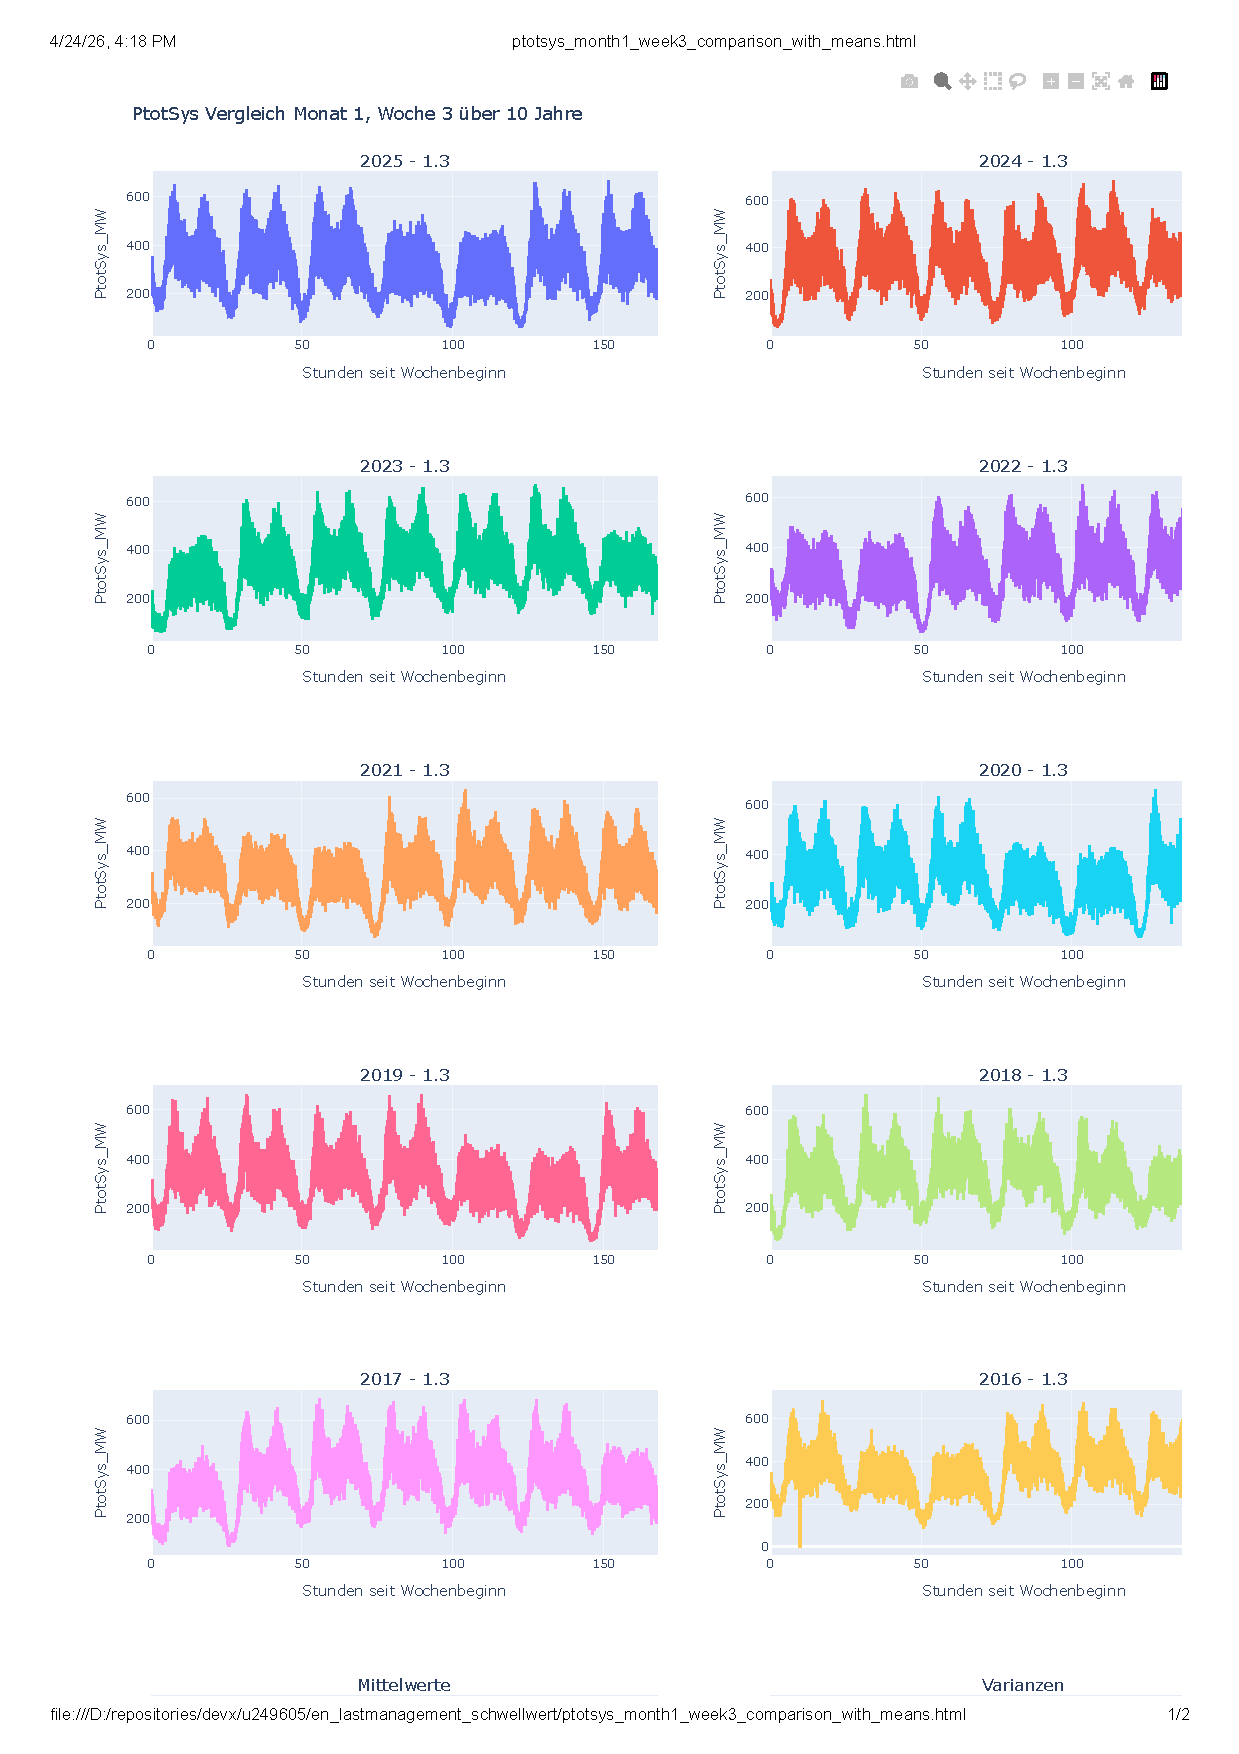
\includegraphics[page=1,scale=0.8,trim={1.2cm 1.4cm 1.2cm 2.2cm},clip]{images/ptotsys_month1_week3_comparison_with_means.html.pdf}
  \caption{Ptotsywerte der letzten 10 Jahre in der 3. Januarwoche.}
\end{figure}
\clearpage
\begin{figure}
  \centering
  \includegraphics[page=2,width=0.95\textwidth,trim={1.2cm 25cm 9.5cm 1.2cm},clip]{images/ptotsys_month1_week3_comparison_with_means.html.pdf}\\[0.8cm]
  \caption{Mittelwerte der Ptotsywerte der letzten 10 Jahre in der 3. Januarwoche, erste Darstellung.}
\end{figure}

\begin{figure}
  \centering
  \includegraphics[page=2,width=0.95\textwidth,trim={12cm 25cm 1.2cm 1cm},clip]{images/ptotsys_month1_week3_comparison_with_means.html.pdf} % trim={<left> <lower> <right> <upper>}
  \caption{Varianz der Ptotsywerte der letzten 10 Jahre in der 3. Januarwoche.}
\end{figure}

Auffaellig sind die erheblichen Unterschiede zwischen den einzelnen Jahren. Die Jahre 2016 und 2017 zeigen deutlich hoehre Mittelwerte (348.16 und 350.38), waehrend die Jahre 2020 und 2021 merklich tiefere Werte aufweisen (304.27 und 304.43). Dies laesst sich wahrscheinlich auf die COVID-19-Pandemie zurueckfuehren, welche einen verkürzten Fahrplan und geaenderte Zugkompositionen zur Folge hatte. Die Reduktion der Ptotsywerte in diesen Jahren deutet auf eine gesamt niedrigere Systemlast hin. Dieses Muster der erhoehten Werte in 2016 und 2017 sowie der reduzierten Werte in 2020 und 2021 zeigt sich konsistent auch in der vierten Juniwoche und deutet auf eine systemweite Auswirkung dieser Effekte hin.

\subsection{Analyse der 4. Juniwoche}
\label{sec:analyse_juni}
In dieser Analyse wird jeweils die vierte Juniwoche der Jahre 2015 bis 2025 betrachtet. Grundlage sind wiederum die taeglichen Ptotsywerte, mit denen die Entwicklung der Schwellwerte ueber den gesamten Zeitraum untersucht wird. Dazu werden sowohl die durchschnittlichen als auch die maximalen Ptotsywerte ausgewertet, um Trends und moegliche Veraenderungen in der Schwellwertsetzung zu identifizieren.
Die folgenden Mittelwerte der Ptotsywerte ergeben sich fuer die vierte Juniwoche in den Jahren 2015 bis 2025:

\begin{table}[H]
  \centering
  \begin{minipage}[t]{0.48\textwidth}
    \centering
    \captionof{table}{Mittelwerte der Ptotsywerte in der 4. Juniwoche}
    \begin{tabular}{lr}
      \toprule
      Jahr & Mittelwert \\
      \midrule
      2025 & 270.634 \\
      2024 & 265.855 \\
      2023 & 266.106 \\
      2022 & 264.347 \\
      2021 & 257.588 \\
      2020 & 250.801 \\
      2019 & 270.958 \\
      2018 & 265.025 \\
      2017 & 275.250 \\
      2016 & 277.329 \\
      \bottomrule
    \end{tabular}
  \end{minipage}
  \hfill
  \begin{minipage}[t]{0.48\textwidth}
    \centering
    \captionof{table}{Varianz der Ptotsywerte in der 4. Juniwoche}
    \begin{tabular}{lr}
      \toprule
      Jahr & Varianz \\
      \midrule
      2025 & 10552.442 \\
      2024 & 9629.283 \\
      2023 & 9860.162 \\
      2022 & 8722.021 \\
      2021 & 8235.471 \\
      2020 & 9184.714 \\
      2019 & 10735.115 \\
      2018 & 9609.851 \\
      2017 & 9946.879 \\
      2016 & 10203.375 \\
      \bottomrule
    \end{tabular}
  \end{minipage}
\end{table}

\begin{figure}
  \centering
  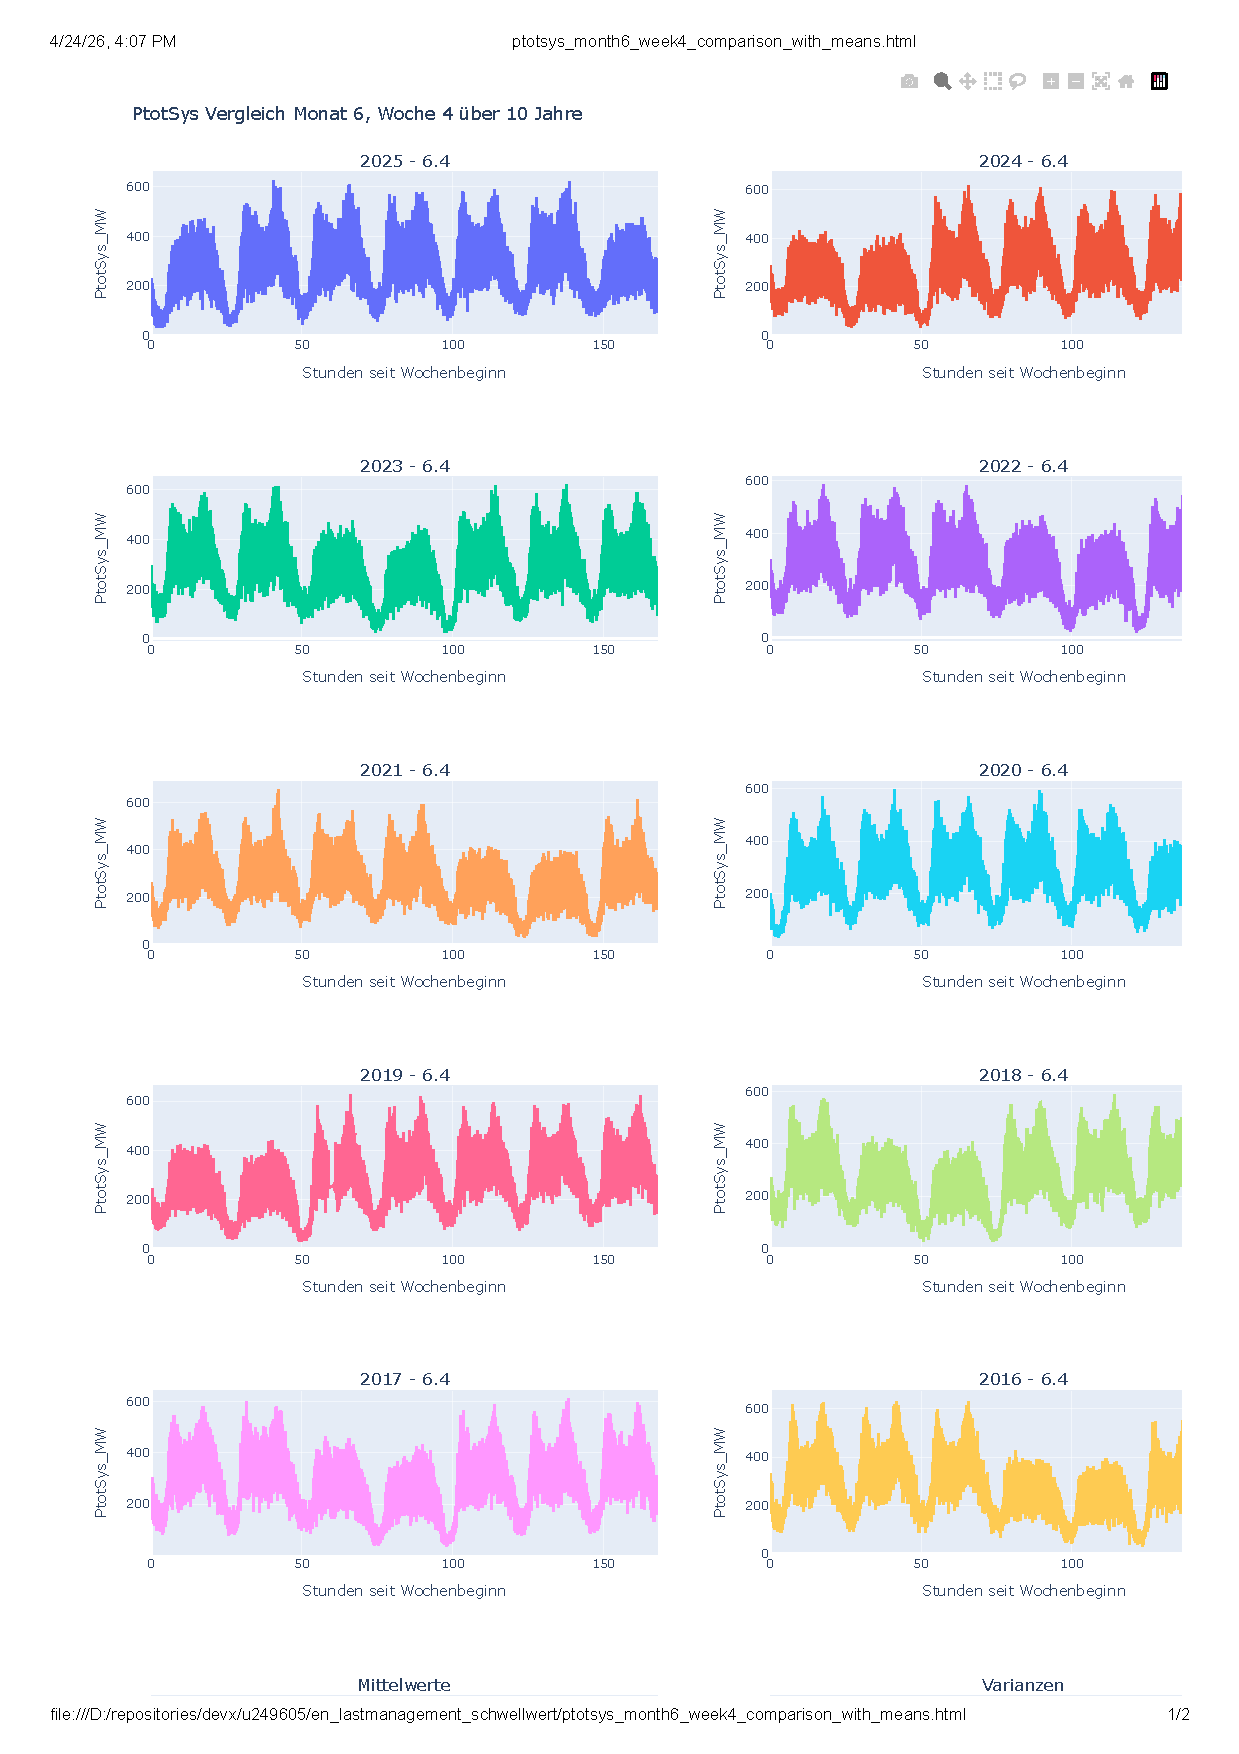
\includegraphics[page=1,scale=0.8,trim={1.2cm 1.4cm 1.2cm 2.2cm},clip]{images/ptotsys_month6_week4_comparison_with_means.html.pdf}
  \caption{Ptotsywerte der letzten 10 Jahre in der 4. Juniwoche.}
\end{figure}
\clearpage
\begin{figure}
  \centering
  \includegraphics[page=2,width=0.95\textwidth,trim={1.2cm 25cm 9.5cm 1.2cm},clip]{images/ptotsys_month6_week4_comparison_with_means.html.pdf}
  \caption{Mittelwerte der Ptotsywerte der letzten 10 Jahre in der 4. Juniwoche.}
\end{figure}

\begin{figure}
  \centering
  \includegraphics[page=2,width=0.95\textwidth,trim={12cm 25cm 1.2cm 1cm},clip]{images/ptotsys_month6_week4_comparison_with_means.html.pdf}
  \caption{Varianz der Ptotsywerte der letzten 10 Jahre in der 4. Juniwoche.}
\end{figure}

Auch in der vierten Juniwoche sind auffaellige Unterschiede zwischen den Jahren erkennbar. Die Jahre 2016 und 2017 weisen mit 277.33 und 275.25 erheblich hoehre Mittelwerte auf, waehrend insbesondere das Jahr 2020 mit einem Mittelwert von 250.80 die niedrigsten Werte zeigt. Die Jahre 2020 und 2021 (250.80 und 257.59) liegen deutlich unter dem Durchschnitt der gesamten Periode, was ebenfalls auf die Auswirkungen der COVID-19-Pandemie zurueckzufuehren ist. Der verkürzter Fahrplan und die Anpassungen in der Zugkomposition bedingt durch die Pandemie fuehrten zu einer reduzierten Systemlast in dieser Woche.

\subsection{Analyse der Januar-Monatswerte}
\label{sec:analyse_januar_monat}
Zusaetzlich zur Wochenbetrachtung werden hier die aggregierten Monatswerte fuer Januar ausgewertet. Die folgenden Kennzahlen (Mittelwert, Varianz, 95\%-Perzentilwert (p95) und 99\%-Perzentilwert (p99)) beziehen sich auf die Jahre 2017 bis 2026.

\begin{table}[H]
  \centering
  \caption{Kennzahlen der Ptotsywerte im Monat Januar}
  \begin{tabular}{lrrrr}
    \toprule
    Jahr & Mittelwert & Varianz & 95\%-Perzentil (p95) & 99\%-Perzentil (p99) \\
    \midrule
    2026 & 307.288 & 10329.212 & 471.635 & 531.967 \\
    2025 & 299.201 & 10061.289 & 459.883 & 521.348 \\
    2024 & 297.364 & 10189.783 & 460.410 & 522.681 \\
    2023 & 296.337 & 10104.641 & 459.263 & 522.586 \\
    2022 & 298.431 & 9641.617 & 456.956 & 515.358 \\
    2021 & 296.043 & 8990.277 & 446.474 & 500.603 \\
    2020 & 294.849 & 9293.838 & 453.354 & 512.554 \\
    2019 & 311.238 & 10115.453 & 474.971 & 532.803 \\
    2018 & 284.746 & 8889.735 & 437.264 & 491.290 \\
    2017 & 328.322 & 10378.154 & 491.835 & 550.242 \\
    \bottomrule
  \end{tabular}
\end{table}

\begin{figure}[H]
  \centering
  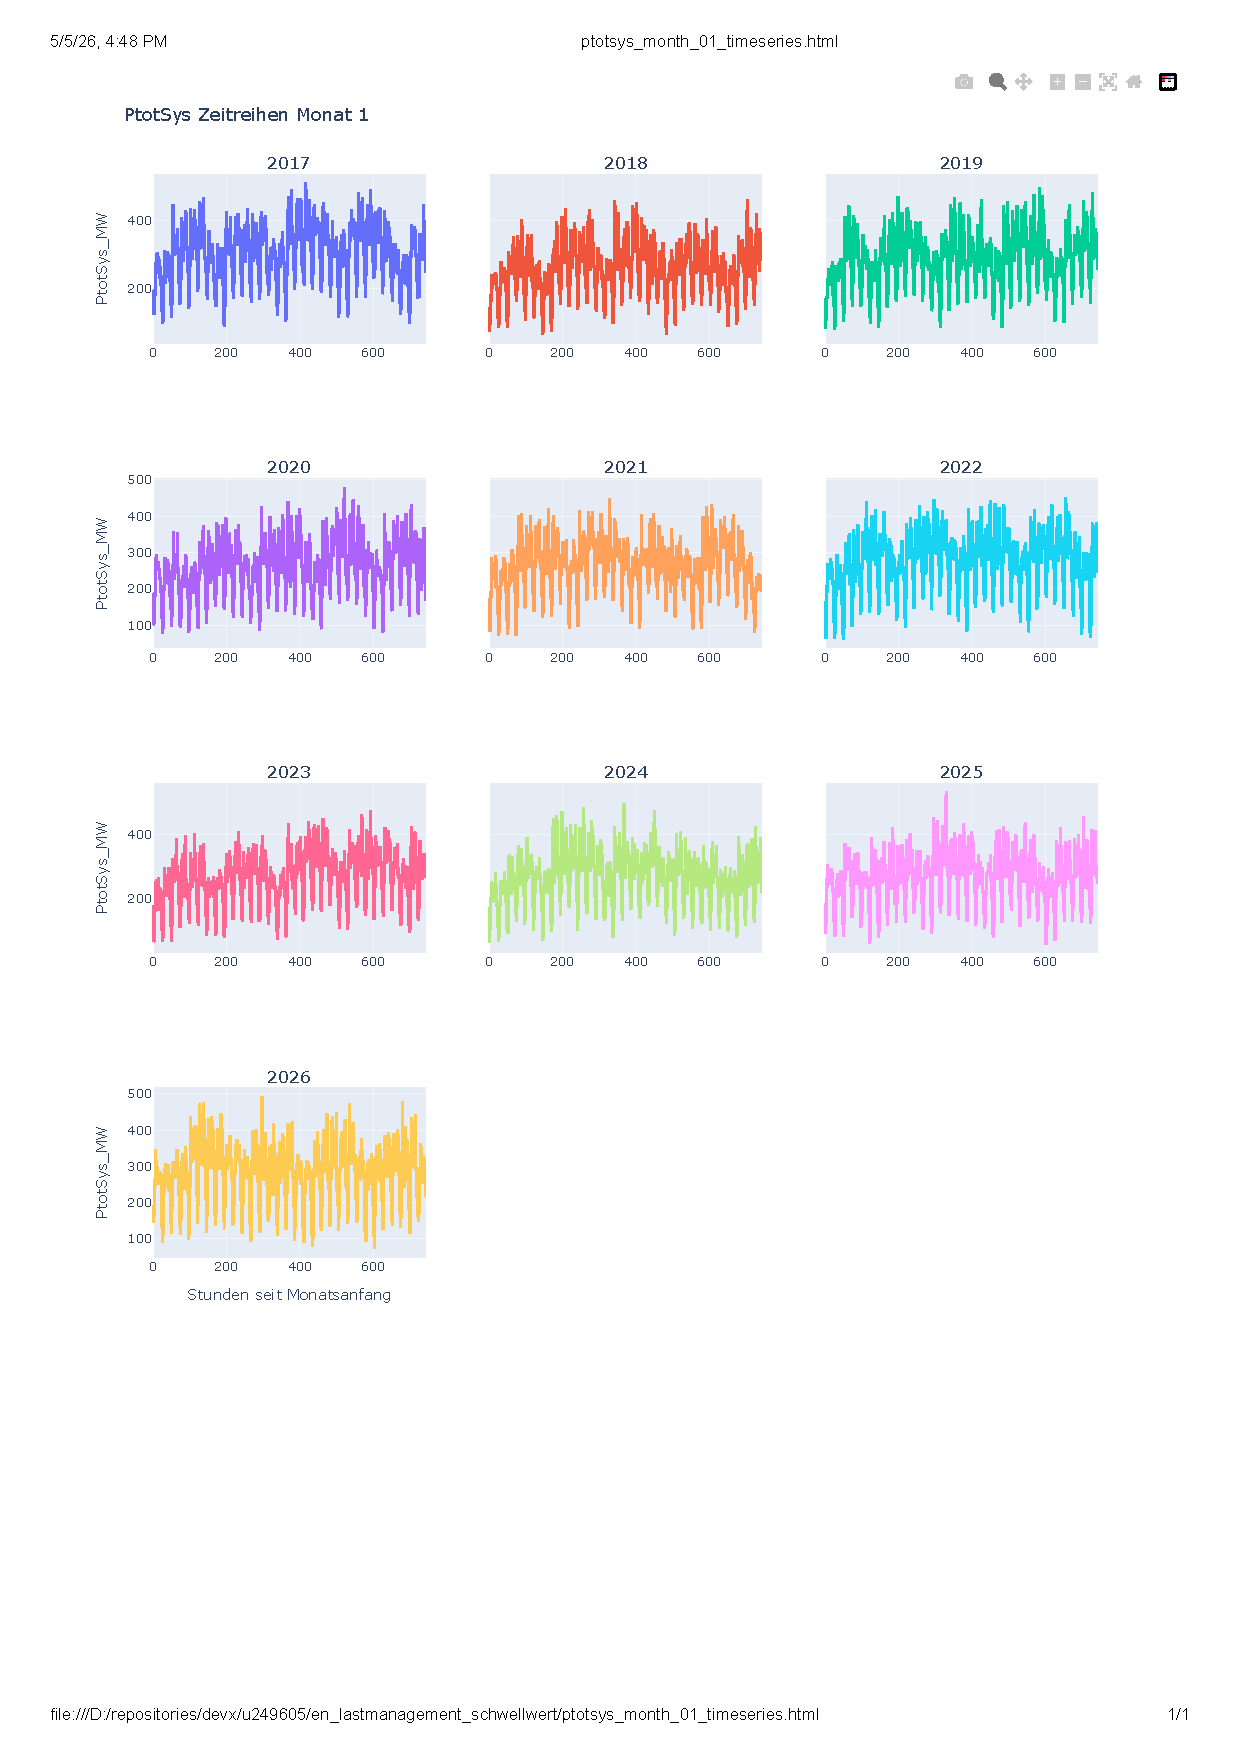
\includegraphics[width=0.95\textwidth,trim={1.2cm 13.0cm 1.2cm 2.1cm},clip]{images/ptotsys_month_01_timeseries.html.pdf}
  \caption{Zeitreihe der Ptotsywerte im Monat Januar (2017 bis 2026).}
\end{figure}

\begin{figure}[H]
  \centering
  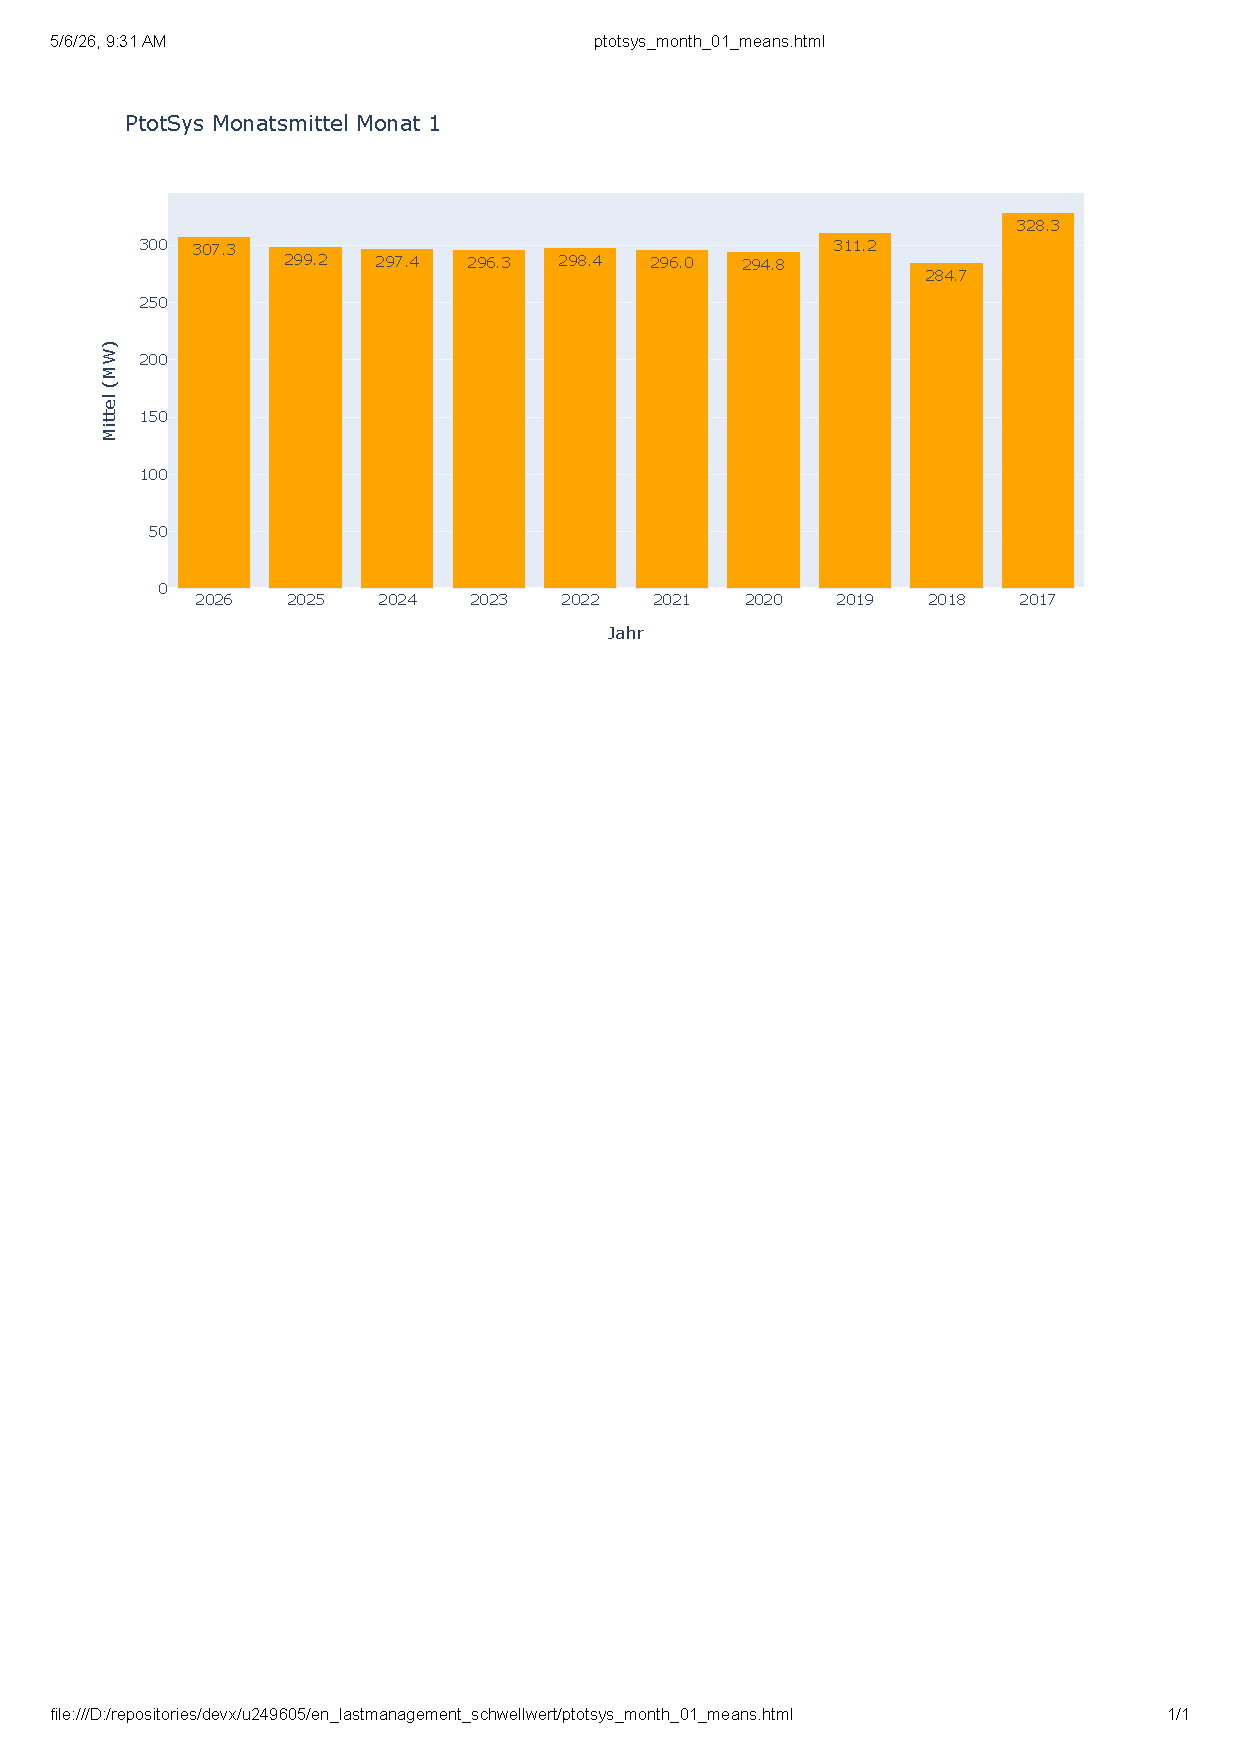
\includegraphics[width=0.95\textwidth,trim={1.2cm 18.9cm 1.2cm 3.1cm},clip]{images/ptotsys_month_01_means.html.pdf}
  \caption{Mittelwerte der Ptotsywerte im Monat Januar (2017 bis 2026).}
\end{figure}

\begin{figure}[H]
  \centering
  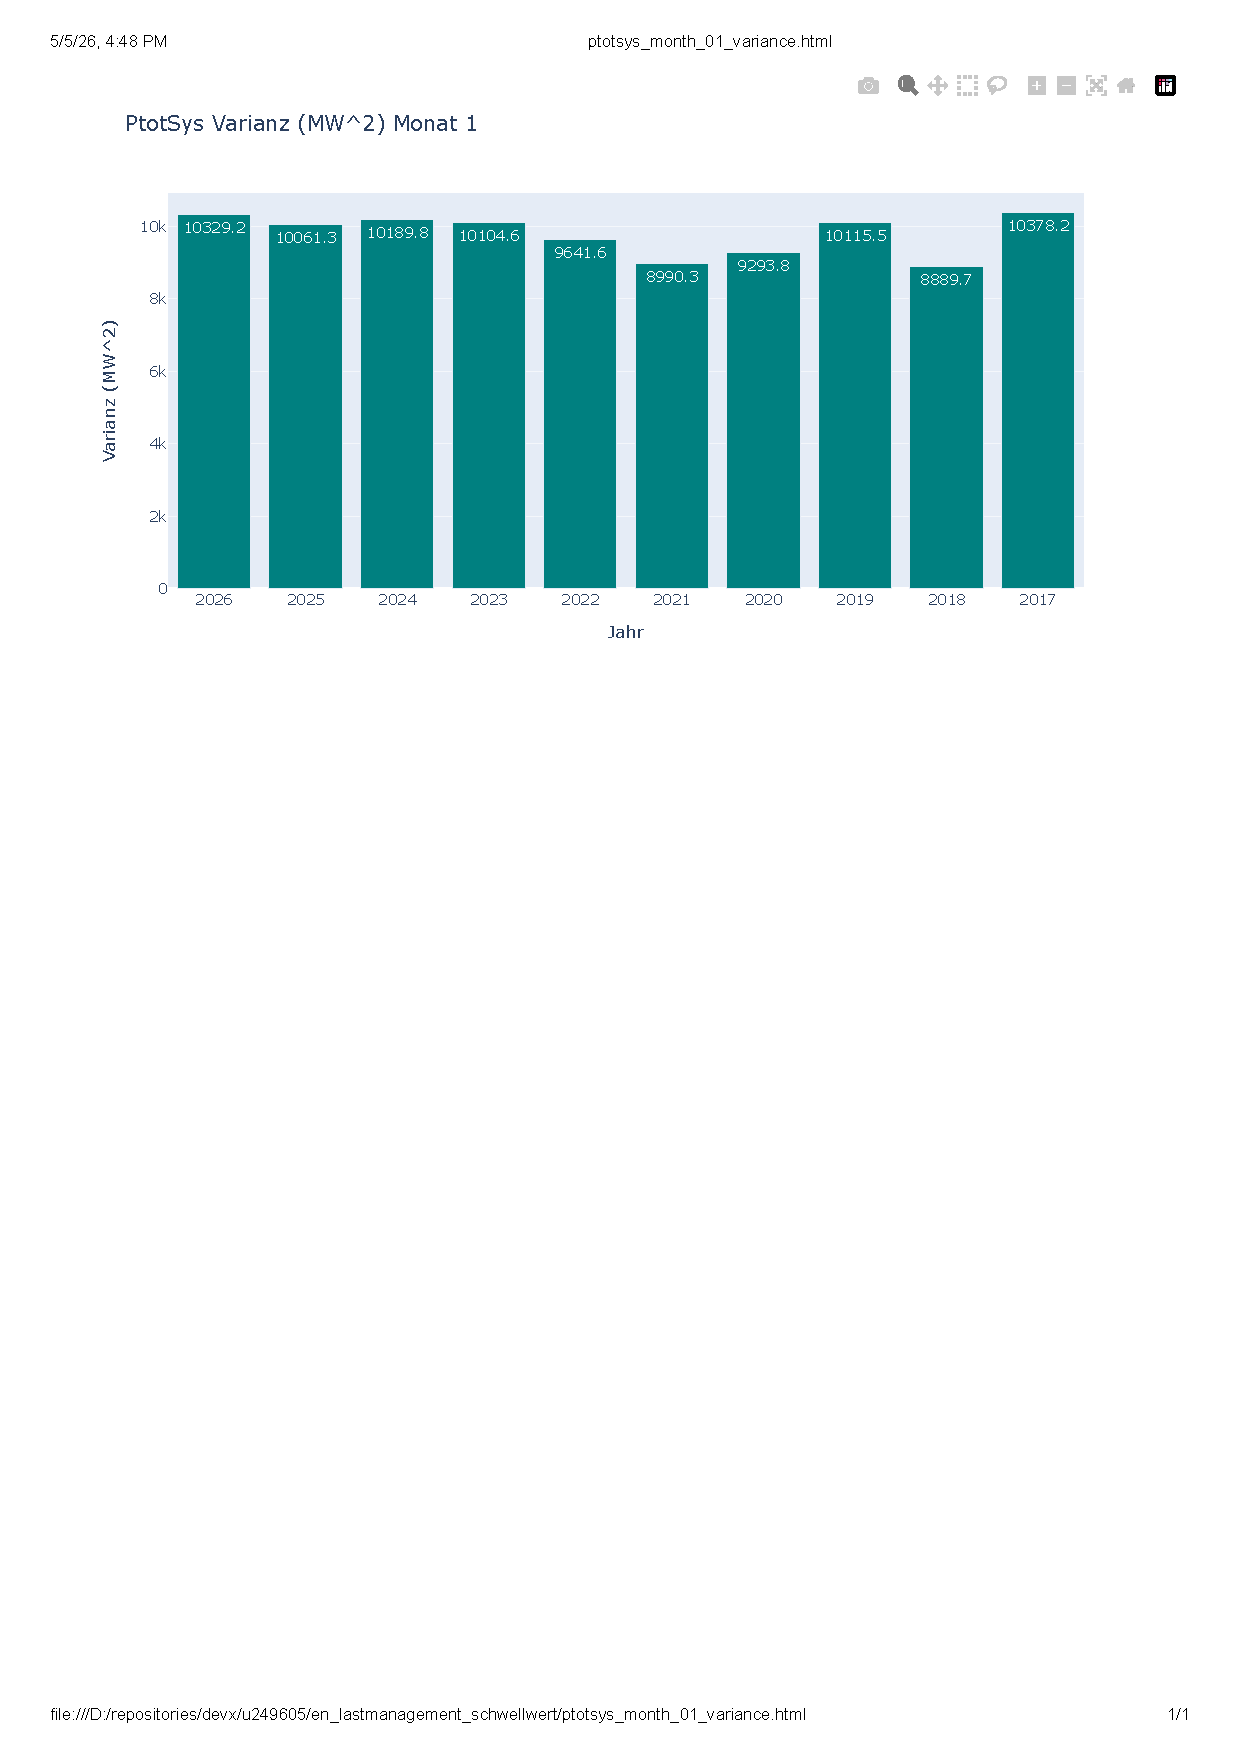
\includegraphics[width=0.95\textwidth,trim={1.2cm 18.6cm 1.2cm 3.1cm},clip]{images/ptotsys_month_01_variance.html.pdf}
  \caption{Varianz der Ptotsywerte im Monat Januar (2017 bis 2026).}
\end{figure}

\begin{figure}[H]
  \centering
  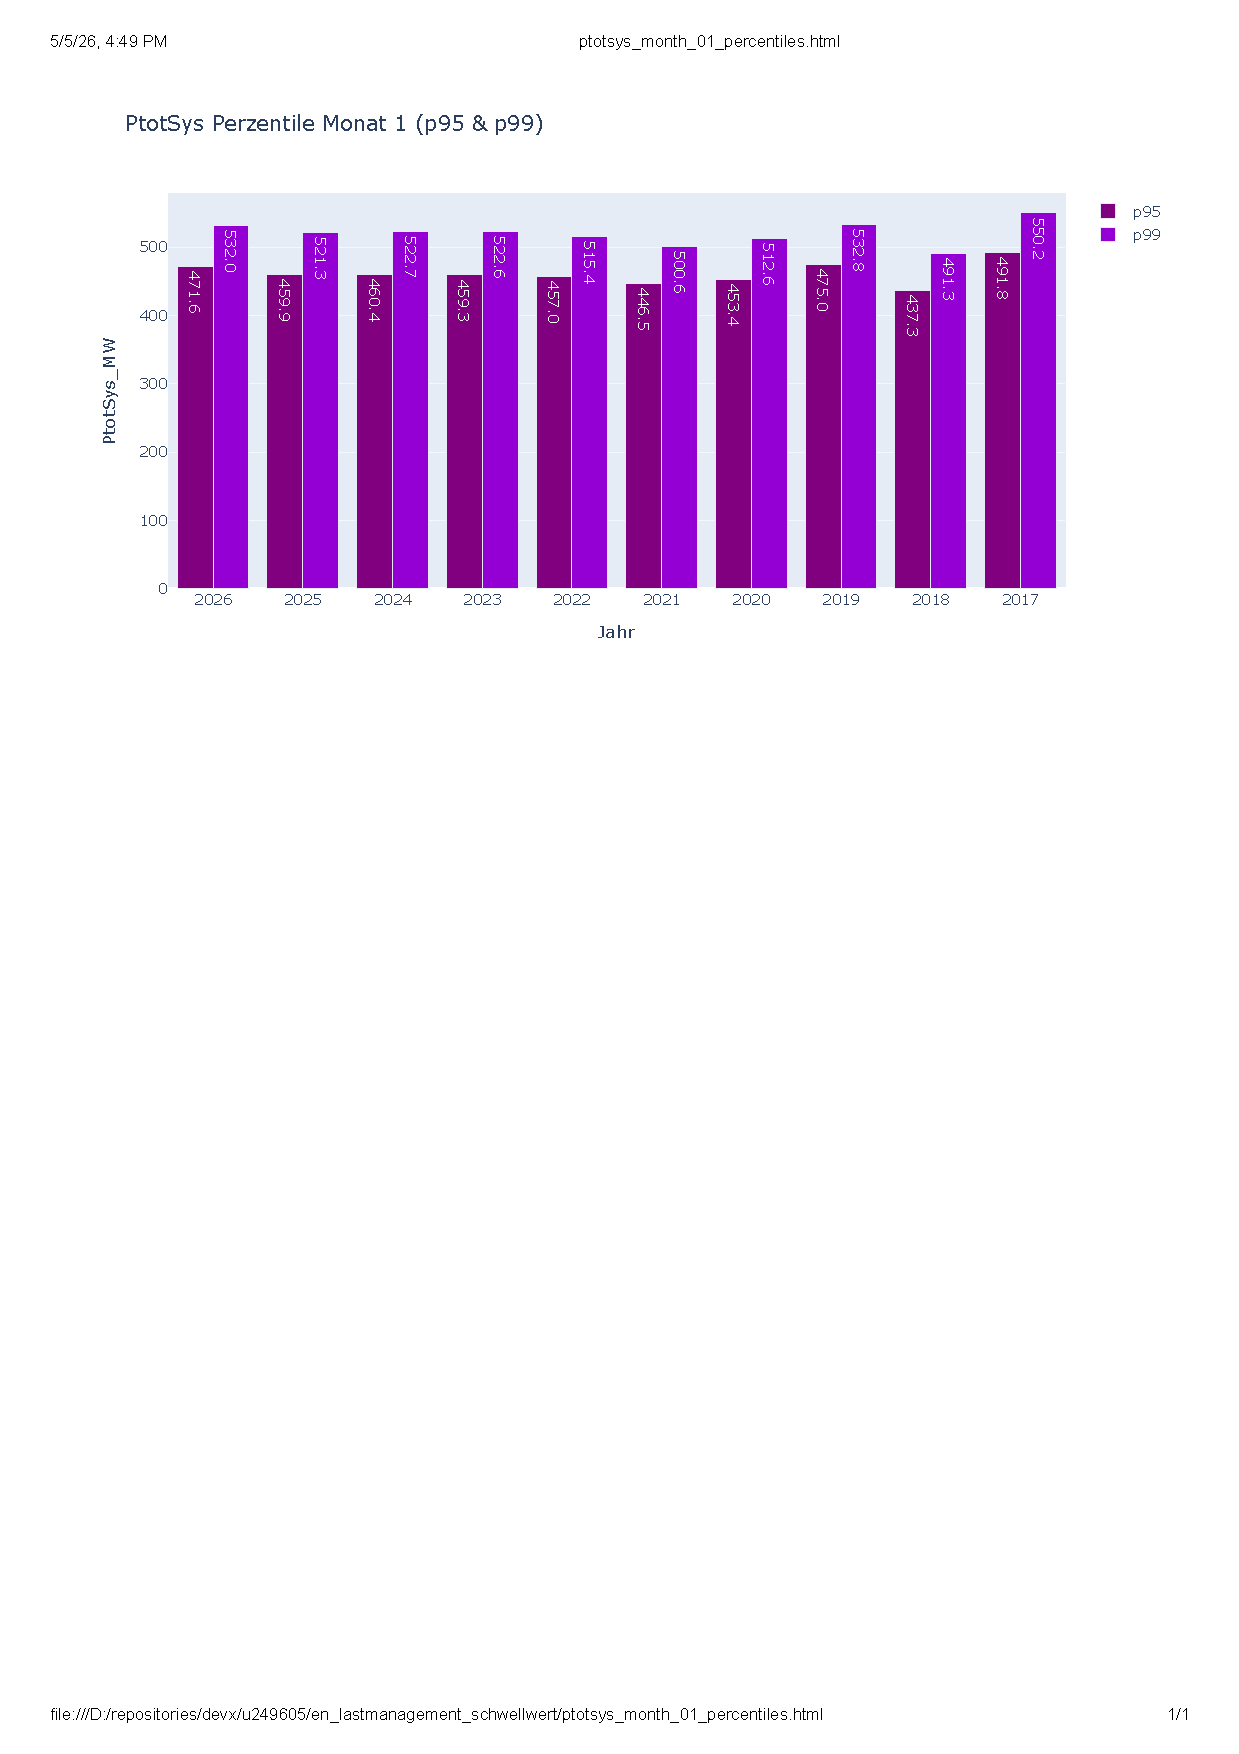
\includegraphics[width=0.95\textwidth,trim={1.2cm 18.6cm 1.2cm 3.1cm},clip]{images/ptotsys_month_01_percentiles.html.pdf}
  \caption{Perzentile: 95\%-Perzentilwert (p95) und 99\%-Perzentilwert (p99) der Ptotsywerte im Monat Januar (2017 bis 2026).}
\end{figure}

Die Januar-Monatswerte zeigen ueber den betrachteten Zeitraum insgesamt ein stabiles Niveau mit erkennbaren Ausreissern in einzelnen Jahren. Insbesondere 2017 und 2019 liegen beim Mittelwert sowie bei den oberen Quantilen ueber dem Grossteil der restlichen Jahre.

\subsection{Analyse der Juni-Monatswerte}
\label{sec:analyse_juni_monat}
Zusaetzlich zur Wochenbetrachtung werden hier die aggregierten Monatswerte fuer Juni ausgewertet. Die folgenden Kennzahlen (Mittelwert, Varianz, 95\%-Perzentilwert (p95) und 99\%-Perzentilwert (p99)) beziehen sich auf die Jahre 2017 bis 2025.

\begin{table}[H]
  \centering
  \caption{Kennzahlen der Ptotsywerte im Monat Juni}
  \begin{tabular}{lrrrr}
    \toprule
    Jahr & Mittelwert & Varianz & 95\%-Perzentil (p95) & 99\%-Perzentil (p99) \\
    \midrule
    2025 & 260.734 & 10209.466 & 420.167 & 481.626 \\
    2024 & 263.199 & 9159.831 & 418.173 & 477.831 \\
    2023 & 265.412 & 9697.577 & 421.479 & 481.944 \\
    2022 & 264.849 & 9126.116 & 413.724 & 470.900 \\
    2021 & 260.294 & 8728.362 & 408.690 & 466.822 \\
    2020 & 243.421 & 8427.585 & 388.567 & 441.135 \\
    2019 & 259.742 & 9471.169 & 416.232 & 474.546 \\
    2018 & 264.655 & 9372.864 & 416.349 & 470.556 \\
    2017 & 269.038 & 9495.503 & 423.489 & 479.271 \\
    \bottomrule
  \end{tabular}
\end{table}

\begin{figure}[H]
  \centering
  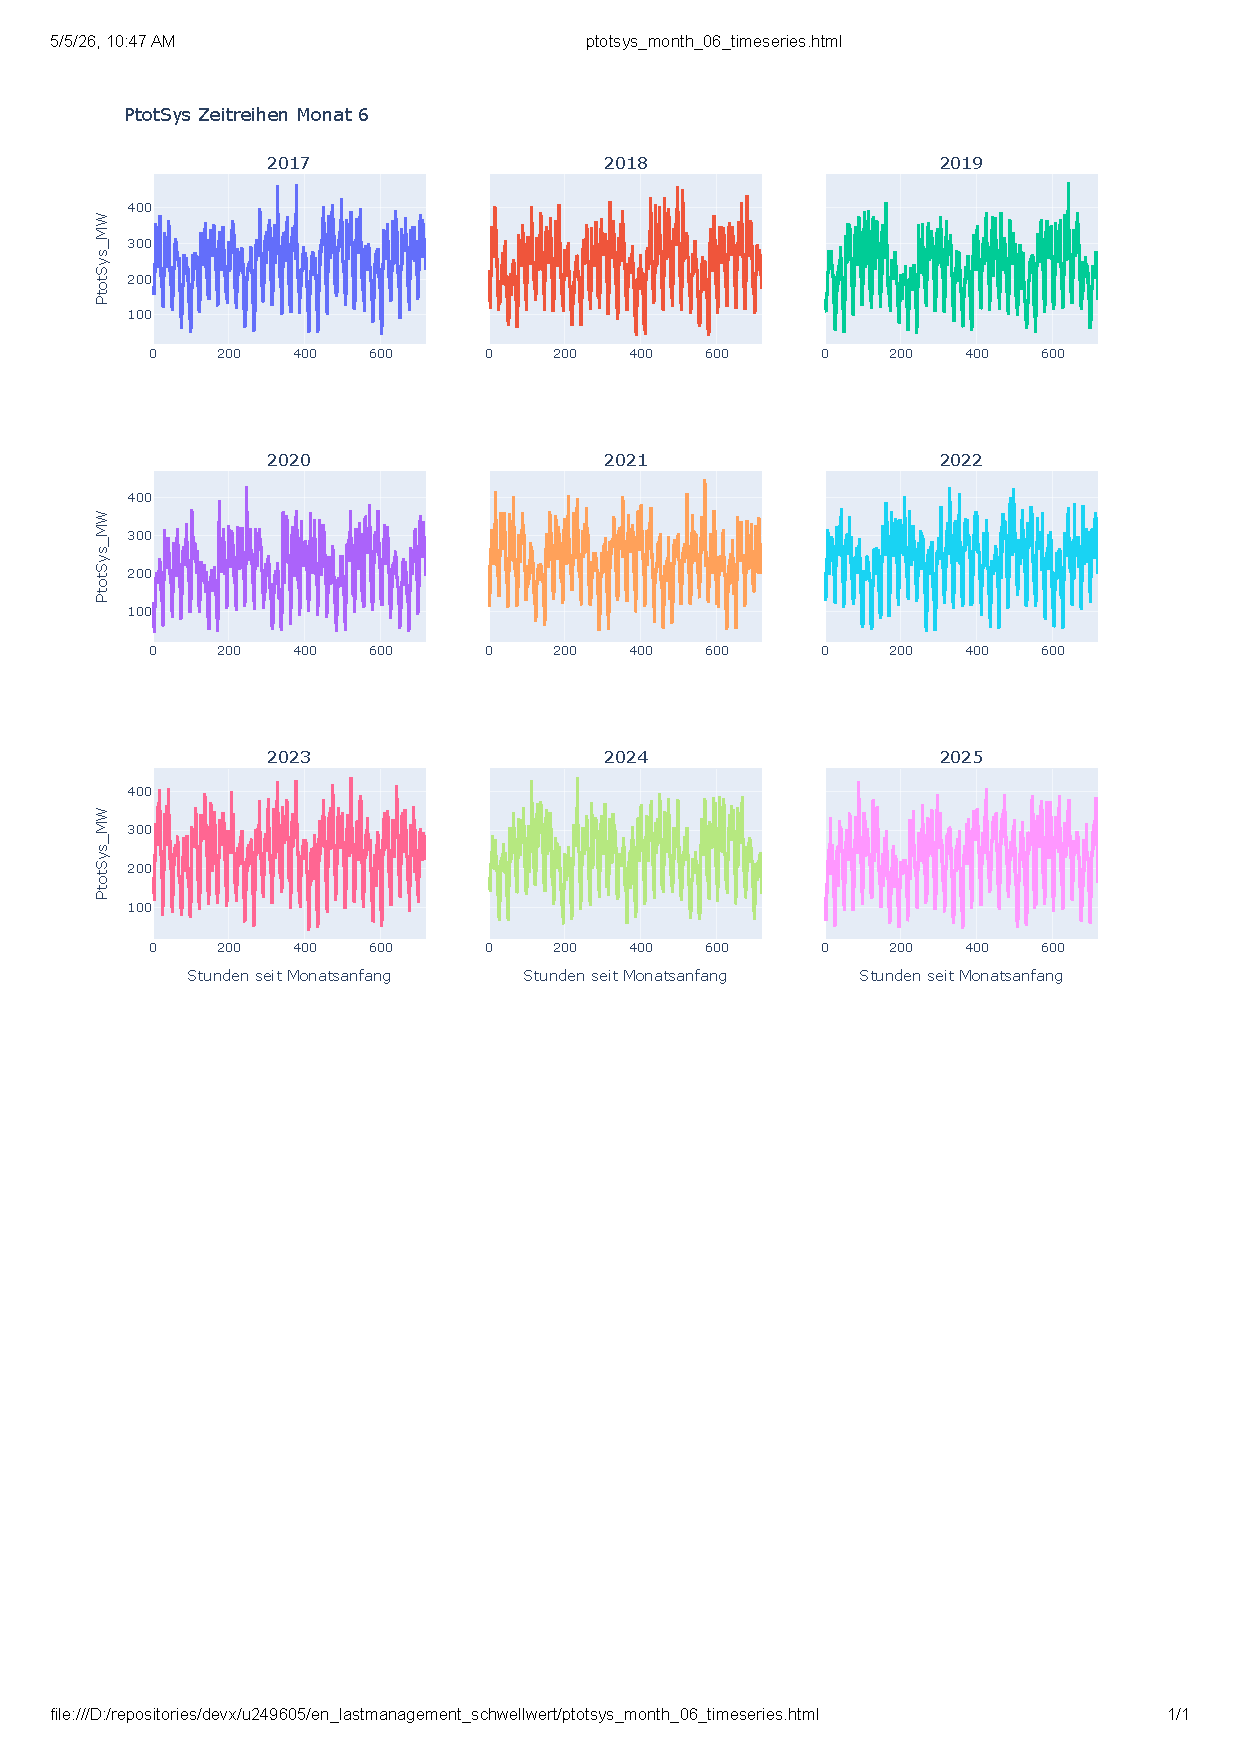
\includegraphics[width=0.95\textwidth,trim={1.2cm 13.0cm 1.2cm 2.1cm},clip]{images/ptotsys_month_06_timeseries.html.pdf}
  \caption{Zeitreihe der Ptotsywerte im Monat Juni (2017 bis 2025).}
\end{figure}

\begin{figure}[H]
  \centering
  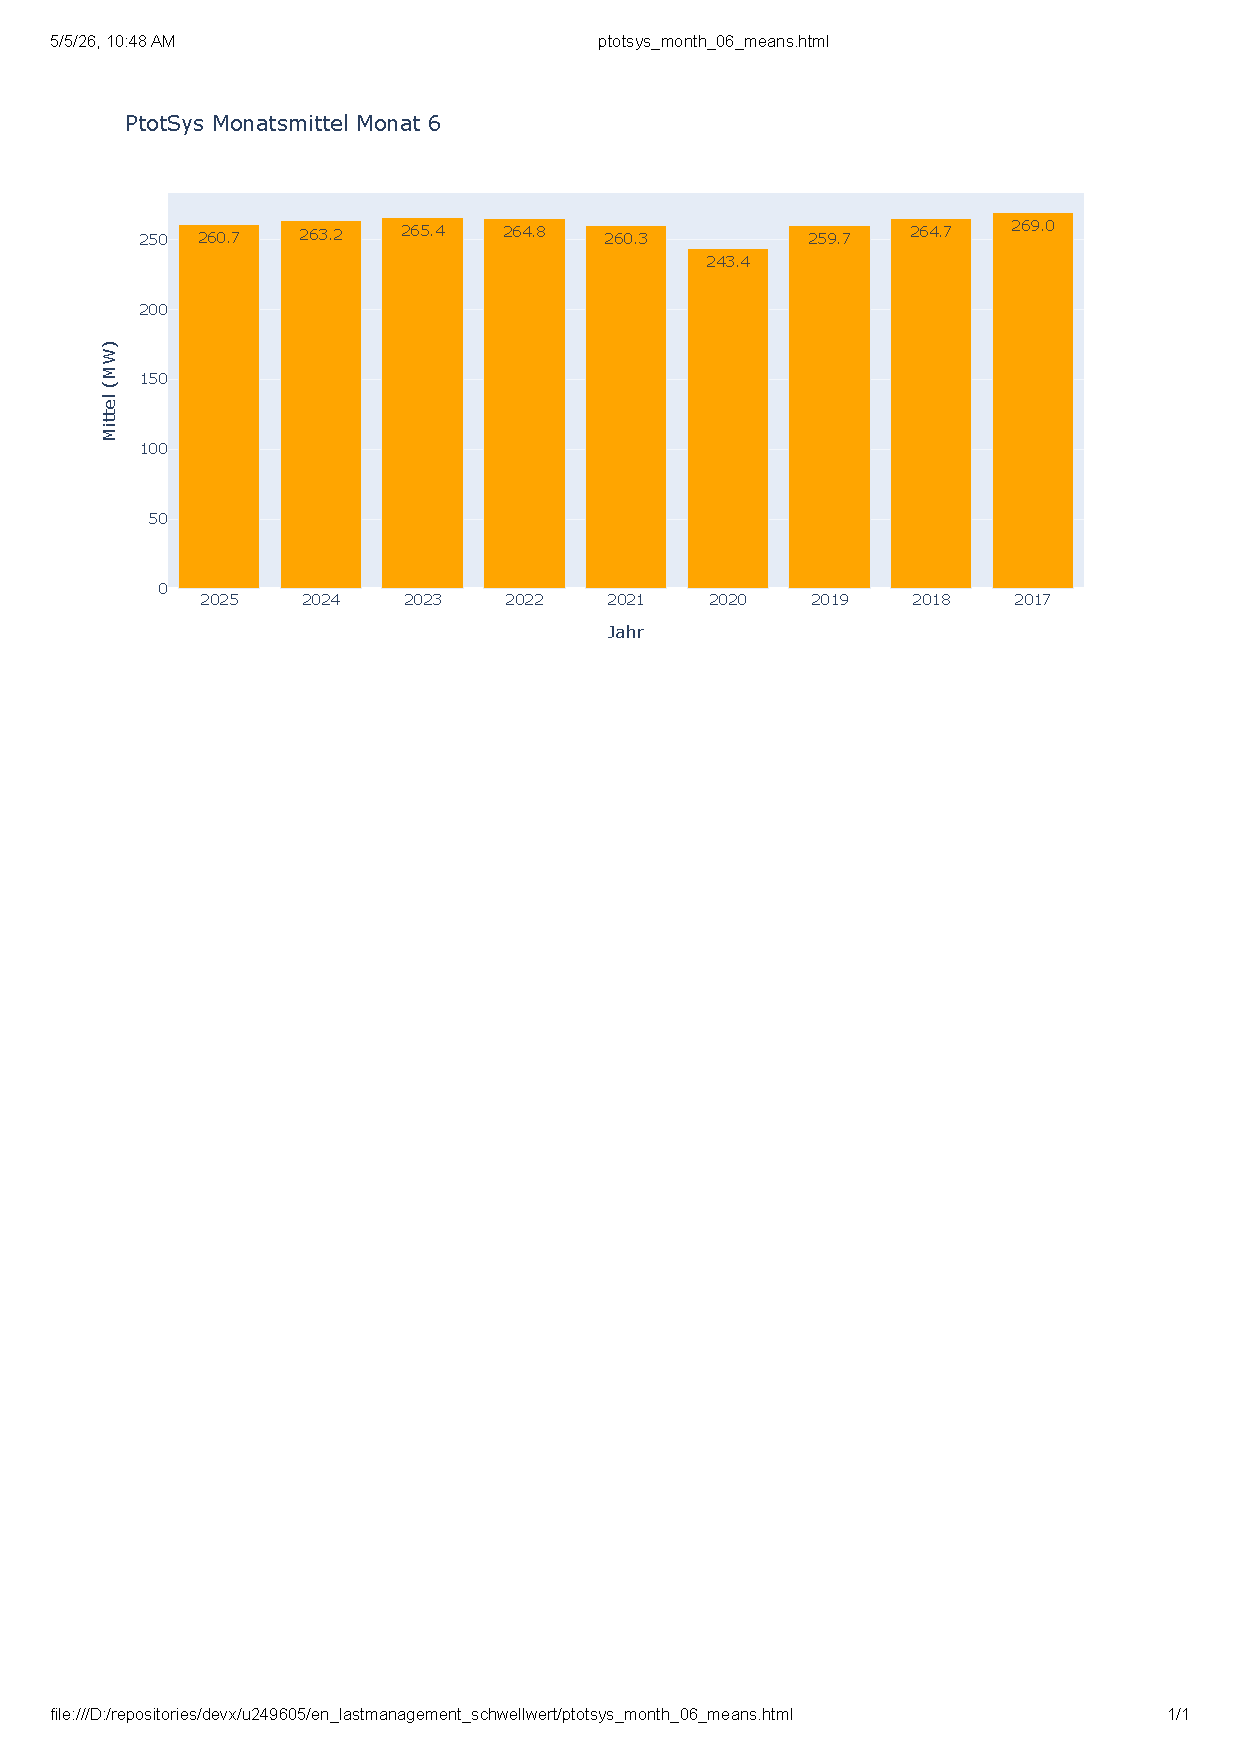
\includegraphics[width=0.95\textwidth,trim={1.2cm 18.9cm 1.2cm 3.1cm},clip]{images/ptotsys_month_06_means.html.pdf}
  \caption{Mittelwerte der Ptotsywerte im Monat Juni (2017 bis 2025).}
\end{figure}

\begin{figure}[H]
  \centering
  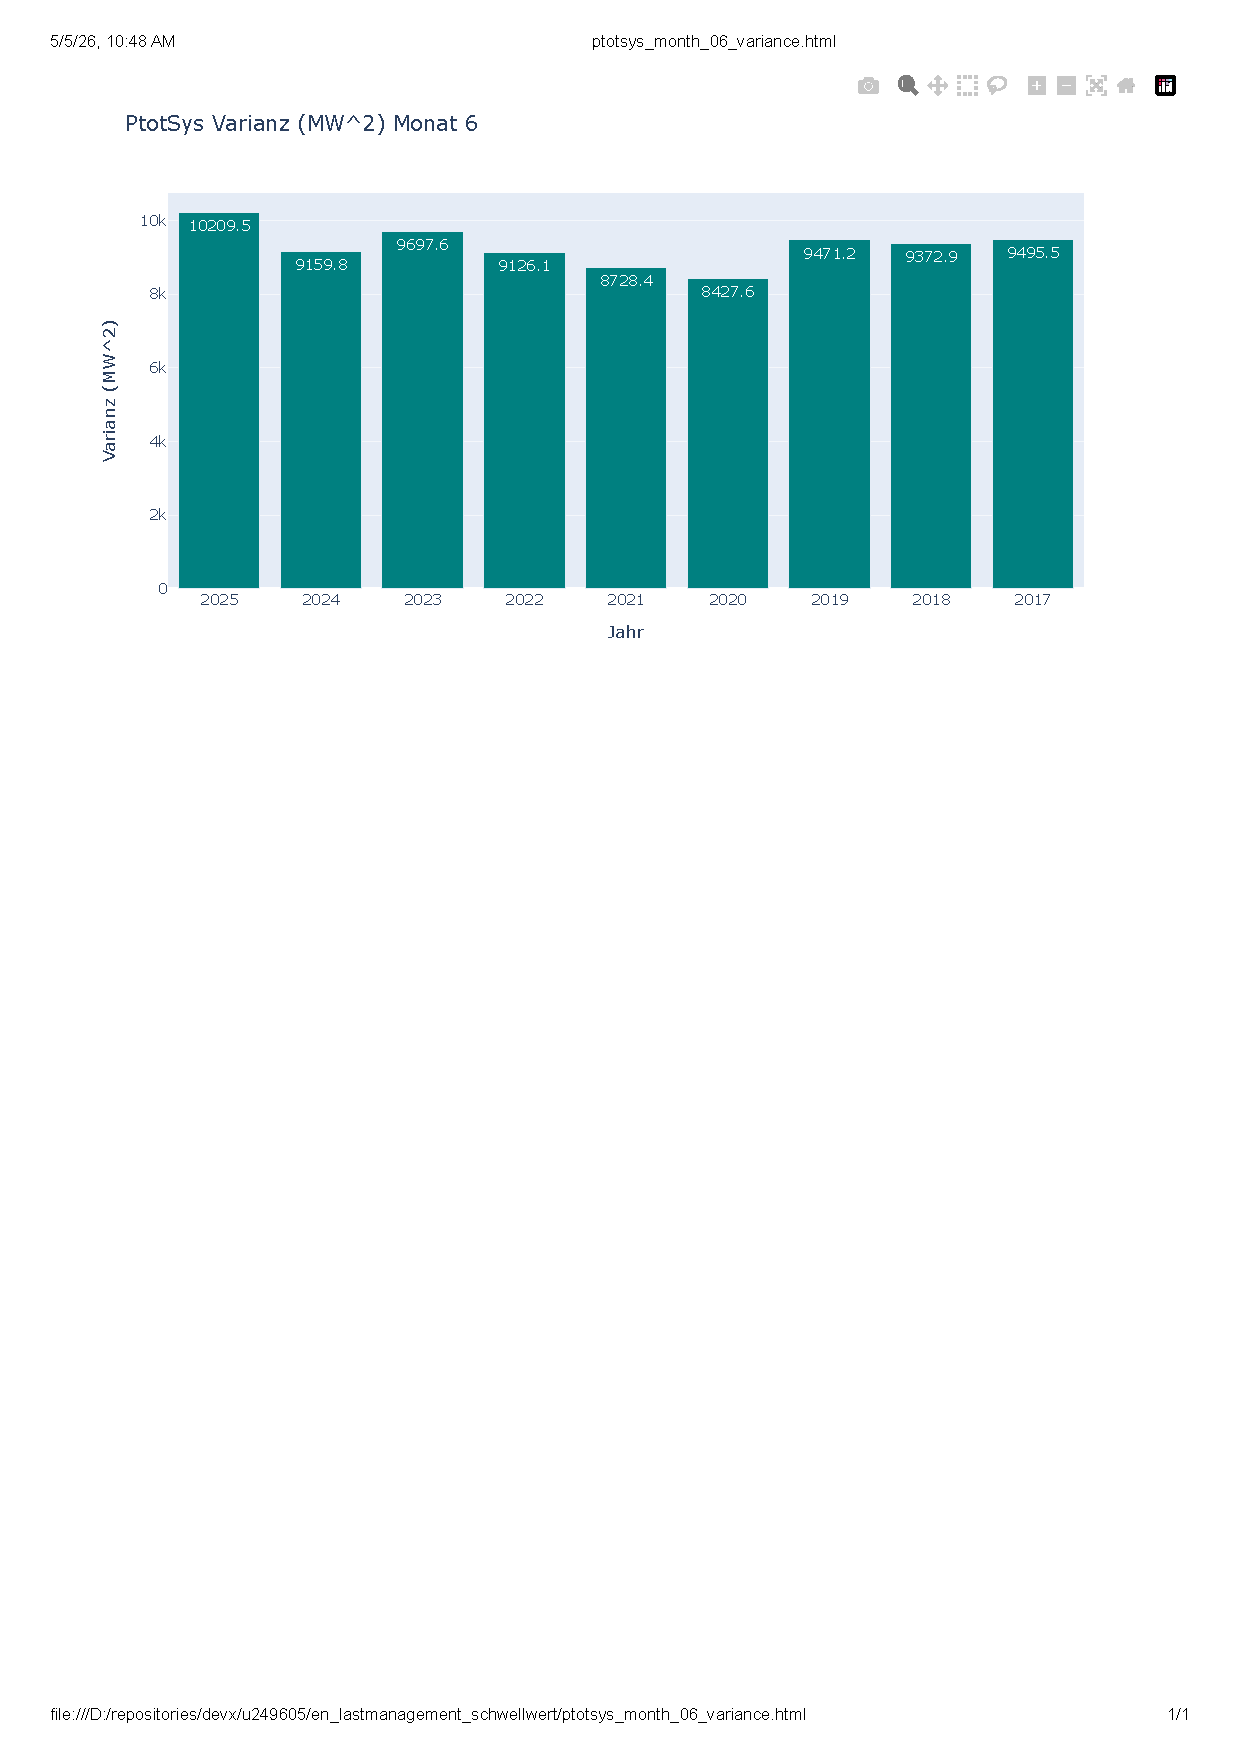
\includegraphics[width=0.95\textwidth,trim={1.2cm 18.6cm 1.2cm 3.1cm},clip]{images/ptotsys_month_06_variance.html.pdf}
  \caption{Varianz der Ptotsywerte im Monat Juni (2017 bis 2025).}
\end{figure}

\begin{figure}[H]
  \centering
  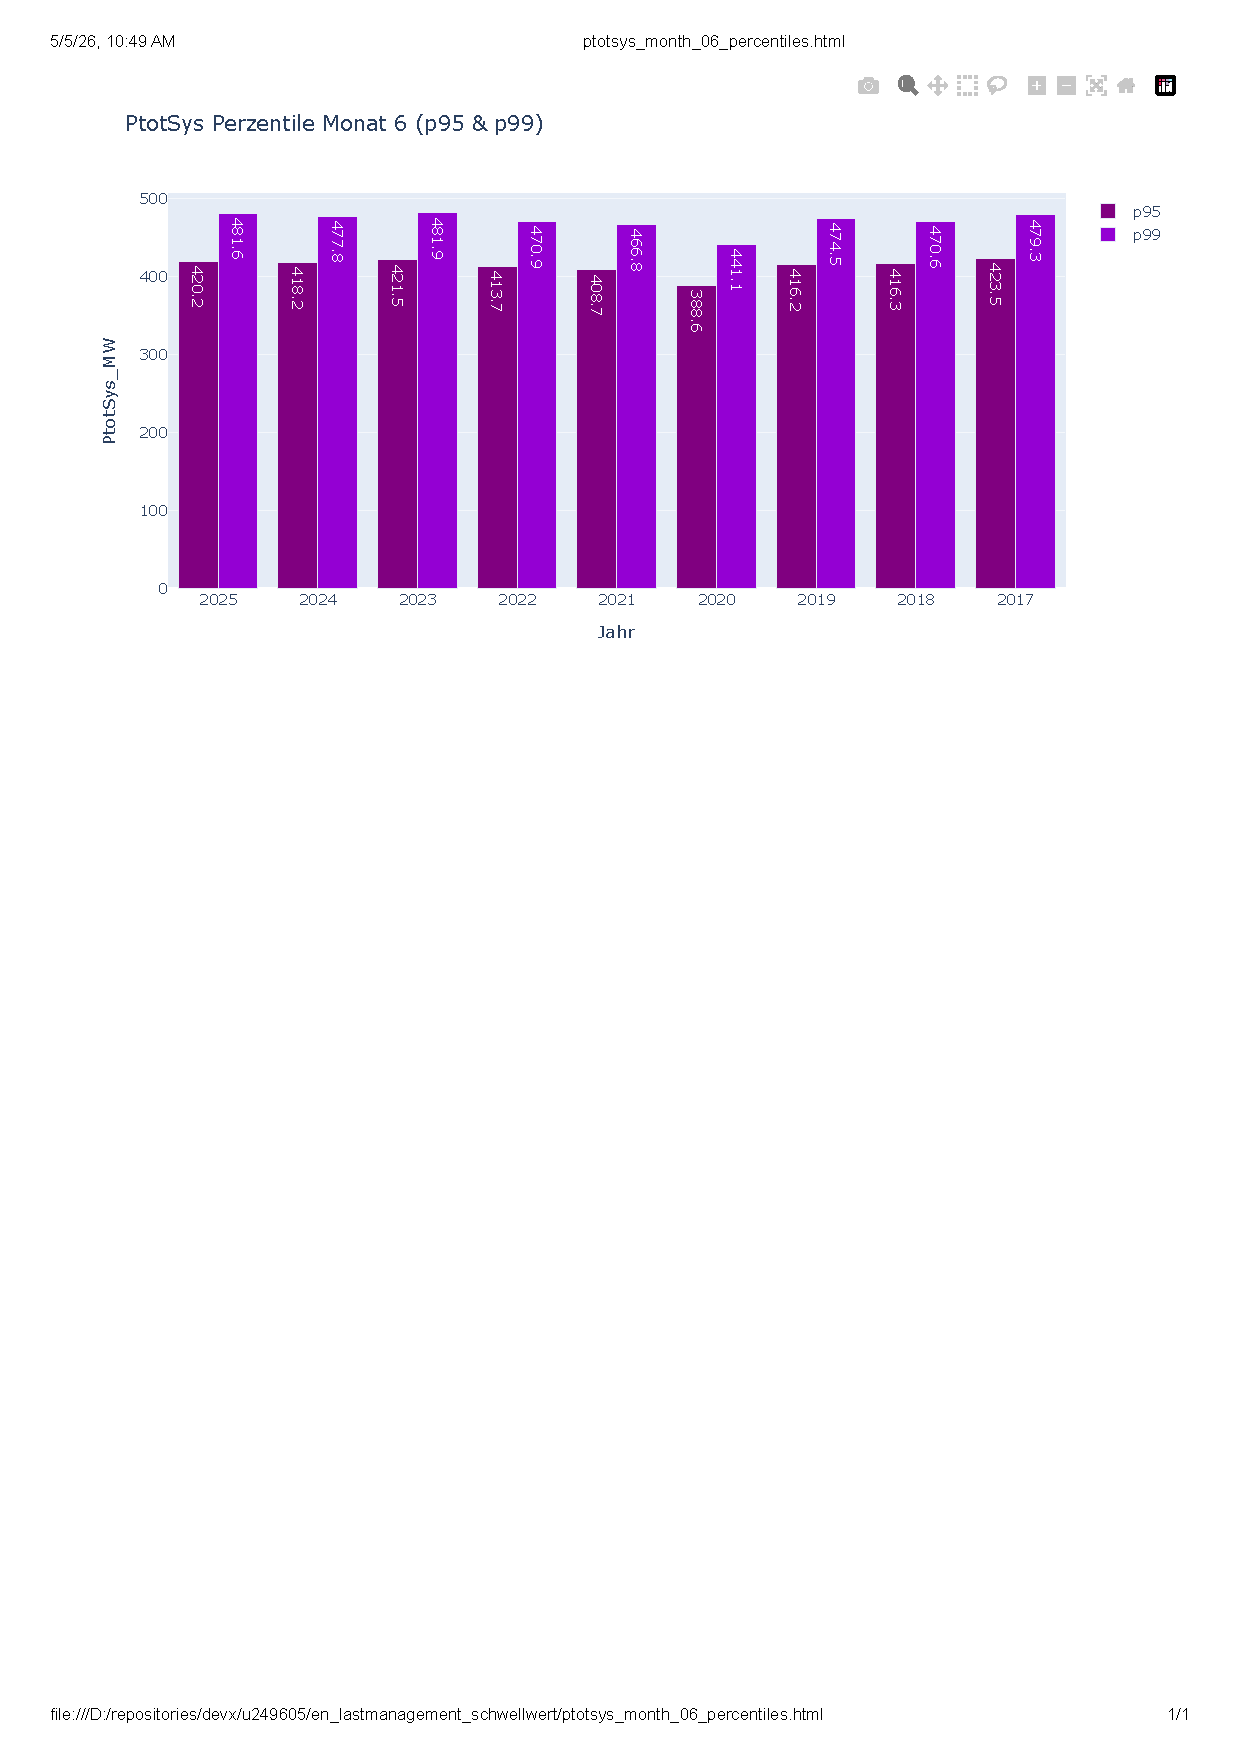
\includegraphics[width=0.95\textwidth,trim={1.2cm 18.6cm 1.2cm 3.1cm},clip]{images/ptotsys_month_06_percentiles.html.pdf}
  \caption{Perzentile: 95\%-Perzentilwert (p95) und 99\%-Perzentilwert (p99) der Ptotsywerte im Monat Juni (2017 bis 2025).}
\end{figure}

Die Juni-Monatswerte zeigen ein insgesamt stabiles Niveau zwischen 2017 und 2025, mit einem klaren Rueckgang im Jahr 2020. Dieser Rueckgang ist sowohl beim Mittelwert als auch bei den hohen Quantilen 95\%-Perzentilwert (p95) und 99\%-Perzentilwert (p99) sichtbar und ist plausibel auf die Auswirkungen der COVID-19-Pandemie zurueckzufuehren. Der waehrend dieser Zeit reduzierte Fahrplan und veraenderte Zugkompositionen fuehrten zu einer niedrigeren Systemlast.

\subsection{Top-3-Peaks pro Jahr}
\label{sec:top3_peaks_jahr}
Zur Einordnung von Extremwerten werden in dieser Subsection die drei hoechsten Ptotsywerte pro Jahr fuer den Zeitraum 2014 bis 2025 dargestellt.

\begin{table}[H]
  \centering
  \caption{Top-3-Peaks der Ptotsywerte pro Jahr (2014 bis 2025)}
  \begin{tabular}{llrr}
    \toprule
    Jahr & Timestamp & Rang im Jahr & Ptotsywert [MW] \\
    \midrule
    2014 & 05.11 & 1 & 660.118 \\
    2014 & 04.12 & 2 & 657.526 \\
    2014 & 03.12 & 3 & 655.701 \\
    2015 & 05.02 & 1 & 697.533 \\
    2015 & 13.02 & 2 & 671.311 \\
    2015 & 05.02 & 3 & 668.553 \\
    2016 & 14.12 & 1 & 714.926 \\
    2016 & 14.01 & 2 & 695.053 \\
    2016 & 15.12 & 3 & 693.241 \\
    2017 & 25.01 & 1 & 705.758 \\
    2017 & 05.07 & 2 & 702.726 \\
    2017 & 06.01 & 3 & 690.851 \\
    2018 & 27.02 & 1 & 711.028 \\
    2018 & 27.02 & 2 & 706.28 \\
    2018 & 27.02 & 3 & 702.622 \\
    2019 & 21.03 & 1 & 745.177 \\
    2019 & 26.11 & 2 & 730.823 \\
    2019 & 26.11 & 3 & 712.23 \\
    2020 & 23.01 & 1 & 662.056 \\
    2020 & 20.01 & 2 & 661.553 \\
    2020 & 04.02 & 3 & 659.86 \\
    2021 & 11.02 & 1 & 700.802 \\
    2021 & 09.03 & 2 & 680.77 \\
    2021 & 07.12 & 3 & 678.708 \\
    2022 & 09.02 & 1 & 761.653 \\
    2022 & 15.12 & 2 & 712.398 \\
    2022 & 14.12 & 3 & 688.306 \\
    2023 & 28.02 & 1 & 694.894 \\
    2023 & 27.01 & 2 & 683.628 \\
    2023 & 09.02 & 3 & 679.428 \\
    2024 & 05.12 & 1 & 716.878 \\
    2024 & 09.12 & 2 & 712.429 \\
    2024 & 24.04 & 3 & 701.378 \\
    2025 & 13.01 & 1 & 736.11 \\
    2025 & 14.02 & 2 & 699.685 \\
    2025 & 18.11 & 3 & 698.89 \\
    \bottomrule
  \end{tabular}
\end{table}

\begin{figure}[H]
  \centering
  \begin{tikzpicture}
    \begin{axis}[
      width=0.95\textwidth,
      height=8.0cm,
      xlabel={Jahr},
      ylabel={Ptotsywert [MW]},
      xmin=2014,
      xmax=2025,
      ymin=0,
      ymax=1000,
      xtick={2014,2015,2016,2017,2018,2019,2020,2021,2022,2023,2024,2025},
      scaled x ticks=false,
      xticklabel style={/pgf/number format/fixed,/pgf/number format/precision=0,/pgf/number format/1000 sep={}},
      grid=major
    ]
      \addplot+[only marks, mark=diamond*, mark options={draw=black}] coordinates {
        (2014,660.118)
        (2014,657.526)
        (2014,655.701)
        (2015,697.533)
        (2015,671.311)
        (2015,668.553)
        (2016,714.926)
        (2016,695.053)
        (2016,693.241)
        (2017,705.758)
        (2017,702.726)
        (2017,690.851)
        (2018,711.028)
        (2018,706.28)
        (2018,702.622)
        (2019,745.177)
        (2019,730.823)
        (2019,712.23)
        (2020,662.056)
        (2020,661.553)
        (2020,659.86)
        (2021,700.802)
        (2021,680.77)
        (2021,678.708)
        (2022,761.653)
        (2022,712.398)
        (2022,688.306)
        (2023,694.894)
        (2023,683.628)
        (2023,679.428)
        (2024,716.878)
        (2024,712.429)
        (2024,701.378)
        (2025,736.11)
        (2025,699.685)
        (2025,698.89)
      };
    \end{axis}
  \end{tikzpicture}
  \caption{Top-3-Peaks der Ptotsywerte pro Jahr als Punktdiagramm.}
\end{figure}

Die Top-3-Peaks bewegen sich in den meisten Jahren in einem Bereich von rund 660 bis 760\,MW. In frueheren Datenstaenden traten in den Jahren 2019, 2016 und 2014 Ausreisser auf, die als potenzielle Fehlmessungen identifiziert wurden. Der Code wurde entsprechend angepasst, um solche Faelle robuster zu erkennen und in der Auswertung angemessen zu behandeln.

\subsection{Varia}
\label{sec:varia}
\begin{itemize}
  \item Es gibt Daten seit dem 12. Mai 2014.
  \item Es gibt keine Daten zum 20.11.2017.
\end{itemize}

\subsection{Temperaturentwicklung und Stabilität der Schwellwerte}
\label{sec:temperatur}

Die Analyse der Schwellwertentwicklung über die Jahre 2015 bis 2026 zeigt bemerkenswert stabile Werte trotz teilweise erheblicher Variabilität. Ein wesentlicher Faktor für diese Stabilität liegt in der relativ konstanten Temperaturentwicklung. Wie die folgende Grafik der globalen Temperaturanomalie demonstriert, ist die Temperatur in den letzten 10 Jahren nur um etwa 1 Grad Celsius angestiegen. Diese begrenzte Temperaturveränderung führt dazu, dass die Schwellwerte sich nicht signifikant nach oben verschieben, sondern eher ein stabiles Verhalten aufweisen.

\begin{figure}[H]
  \centering
  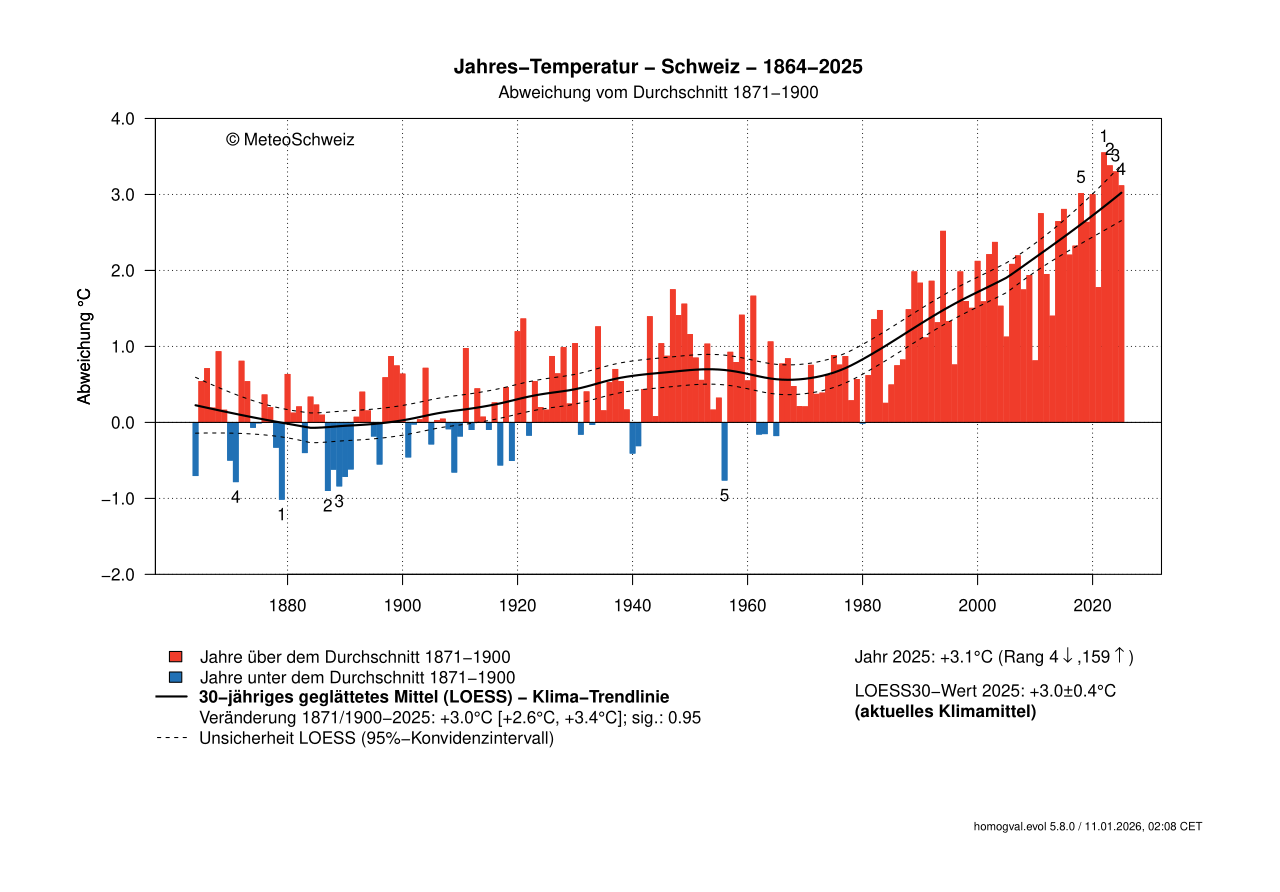
\includegraphics[width=0.95\textwidth]{images/climate-webimage_temperature_loess_de.png}
  \caption{Temperaturanomalie seit 1901 bis heute. Der Fokus liegt auf den letzten 10 Jahren, in denen die Temperatur um etwa 1 Grad Celsius angestiegen ist. Diese begrenzte Temperaturveränderung erklärt die stabilen Schwellwerte in der Analysepeiode. \\ \small Quelle: MeteoSchweiz, \url{https://www.meteoschweiz.admin.ch/service-und-publikationen/applikationen/ext/climate-evolution-series-public.html}}
\end{figure}

Der stabile Temperaturtrend steht in Einklang mit den beobachteten Schwellwertmustern. Während exogene Schocks wie die COVID-19-Pandemie zu kurzfristigen Reduktionen der Systemlast führten, bleibt der langfristige Trend durch die moderate Temperaturentwicklung geprägt. Dies unterstreicht die Bedeutung von Klimafaktoren bei der Schwellwertsetzung und deren Projektion in die Zukunft.

Der Einfluss der Temperatur auf den Energiebedarf ist dabei erheblich: Im Heizbereich bewirkt eine Temperaturänderung von 1\,°C eine Verschiebung der Systemlast von rund 10\,MW, während im Kühlbereich ein Grad Unterschied eine Veränderung von 3–4\,MW verursacht. Diese Sensitivitäten verdeutlichen, warum selbst moderate Klimaveränderungen langfristig zu einer spürbaren Verschiebung der Schwellwerte führen können.

\section{Ergebnisse}
\label{sec:ergebnisse}

\section{Diskussion}
\label{sec:diskussion}

\section{Fazit und Ausblick}
\label{sec:fazit}

% Anhang
\appendix
\section{Anhang A: Ergänzende Tabellen}
\label{app:tabellen}
Zusätzliche Tabellen und Materialien.

% Literaturverzeichnis
\clearpage
\printbibliography[heading=bibintoc,title={Literaturverzeichnis}]

\end{document}
